% Two-panel entropy bookkeeping for melting ice: the environment gives up heat
% (S_env down by Q/T_env), the ice absorbs it (S_ice up by Q/T_ice). Arrow SIZE
% carries the physics: when T_env < T_ice the environment's loss dominates and
% melting is entropically unfavorable; when T_env > T_ice the ice's gain wins.
% alt: Two panels showing an ice cube inside an environment box absorbing
%   heat. Left: when the environment is colder than the ice, a large downward
%   arrow on the environment's entropy outweighs a small upward arrow on the
%   ice's entropy, so melting is unfavorable. Right: when the environment is
%   hotter, the arrow sizes reverse and melting is favorable.
% width: 620
\ifnum\pdfoutput>0
  \documentclass[tikz,border=3pt]{standalone}         % pdflatex → PDF proof
\else
  \documentclass[tikz,border=3pt,dvisvgm]{standalone} % latex   → web SVG
\fi
% Shared setup for all site figures — \input by every figures/*.tex.
% Change the palette, font size, or driver logic HERE and every figure inherits
% it on next rebuild. See src/assets/blog/README.md for the full workflow.
%
% NOTE: this file is \input AFTER \documentclass (it needs amsmath/tikz loaded),
% but the \documentclass line itself carries the driver switch and must stay in
% each figure — see _template.tex. Keep figure .tex files starting from that
% template so the driver logic is never forgotten.

\usepackage{amsmath}

% --- Palette: sentinel hexes = the LIGHT-theme values from DESIGN.md. ----------
% The PDF proof / Overleaf output therefore look like the light rendering, and
% fig.sh rewrites each hex to its themed CSS variable in the web SVG:
%   ink    #000000 -> var(--color-text-main, currentColor)   (also all black strokes)
%   accent #003366 -> var(--color-accent, #003366)
%   muted  #555555 -> var(--color-text-muted, #555555)
%   figred #b91c1c -> var(--fig-red, #b91c1c)
%   figblue   #1d4ed8 -> var(--fig-blue, #1d4ed8)
%   figorange #c2410c -> var(--fig-orange, #c2410c)
\definecolor{ink}{HTML}{000000}
\definecolor{accent}{HTML}{003366}
\definecolor{muted}{HTML}{555555}
\definecolor{figred}{HTML}{B91C1C}
\definecolor{figblue}{HTML}{1D4ED8}
\definecolor{figorange}{HTML}{C2410C}

% --- Figure body font size = site body text. ---------------------------------
% The site renders body text at 18px ≈ 13.5pt. dvisvgm emits the SVG at its
% intrinsic point size and <Figure> shows it ~1:1, so to make figure labels match
% surrounding prose we set the figure's \normalsize to 13.5/16pt. Individual
% labels can still deviate with font=\small / font=\large as needed. Computer
% Modern matches the KaTeX body math, so $dg_p(v)$ reads identically in both.
\newcommand{\figfontsize}{\fontsize{13.5}{16}\selectfont}

% Apply it as the default font for every tikzpicture, plus sane global defaults.
% Dimension figures in mm (x=1mm,y=1mm) so geometry and this pt-based text stay
% independent — scale the drawing by editing coordinates, not the type size.
\tikzset{
  every picture/.style = {font=\figfontsize, line join=round},
  edge/.style          = {line width=1pt},
  hair/.style          = {line width=1pt},
}

\usetikzlibrary{decorations.pathmorphing}

\begin{document}
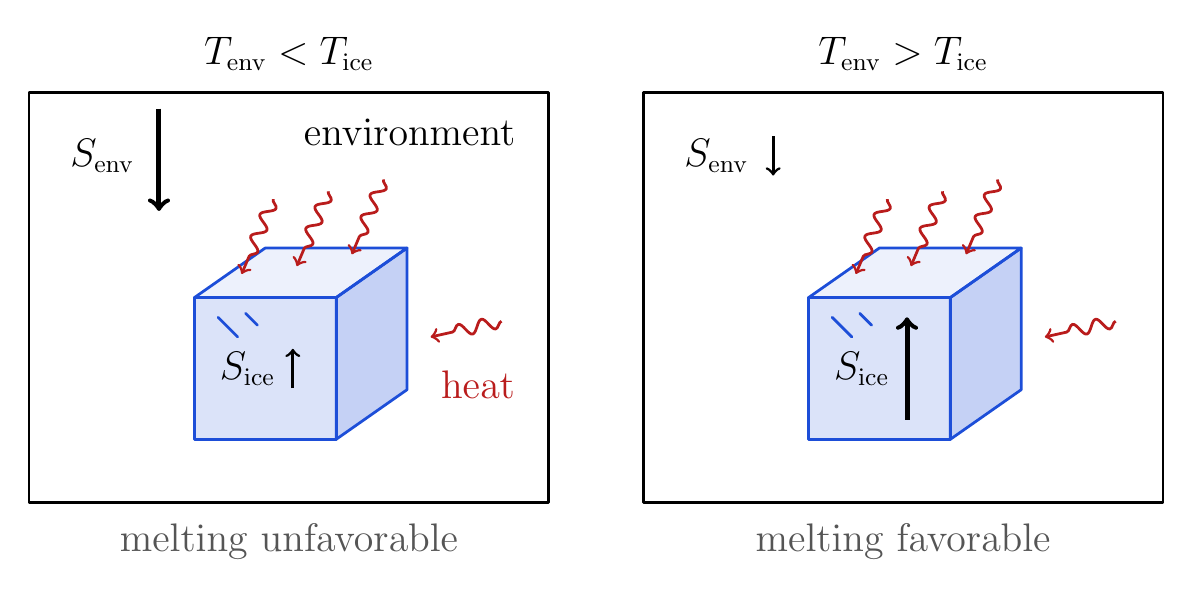
\begin{tikzpicture}[x=1mm, y=1mm]
  % Isometric-ish projection for the ice cube (same setup as cube-x3).
  \def\ax{1}\def\ay{0}      % right
  \def\bx{0}\def\by{1}      % up
  \def\cx{0.5}\def\cy{0.35} % depth (foreshortened)
  \newcommand{\Q}[3]{({(#1)*\ax + (#2)*\bx + (#3)*\cx}, {(#1)*\ay + (#2)*\by + (#3)*\cy})}

  \tikzset{
    % Icy translucent tint over the page bg, one depth per face (top catches
    % light, right sits in shade) so the cube reads as frosted glass. Tint is
    % figblue so it flips with the theme; nothing sits behind the cube, so a
    % translucent fill is safe here (no occlusion needed).
    icetop/.style   = {draw=figblue, edge, fill=figblue, fill opacity=0.08},
    icefront/.style = {draw=figblue, edge, fill=figblue, fill opacity=0.16},
    iceright/.style = {draw=figblue, edge, fill=figblue, fill opacity=0.26},
    heat/.style     = {figred, edge, ->,
                       decorate, decoration={snake, amplitude=0.8mm,
                                             segment length=3mm, post length=2mm}},
    bigarrow/.style   = {ink, line width=1.8pt, ->},
    smallarrow/.style = {ink, line width=1pt, ->},
  }
  \def\X{18}   % ice cube edge (mm)

  % One panel = environment box + ice cube + heat arrows. Entropy arrows differ
  % per panel, so they're drawn outside this macro.
  % \panel{label-env? 1/0}
  \newcommand{\panel}[1]{%
    \draw[edge, ink] (0,0) rectangle (66,52);
    \begin{scope}[shift={(21,8)}]
      % faces drawn individually so each carries its own tint depth
      \filldraw[icefront] \Q{0}{0}{0} -- \Q{\X}{0}{0} -- \Q{\X}{\X}{0} -- \Q{0}{\X}{0} -- cycle;
      \filldraw[icetop]   \Q{0}{\X}{0} -- \Q{\X}{\X}{0} -- \Q{\X}{\X}{\X} -- \Q{0}{\X}{\X} -- cycle;
      \filldraw[iceright] \Q{\X}{0}{0} -- \Q{\X}{\X}{0} -- \Q{\X}{\X}{\X} -- \Q{\X}{0}{\X} -- cycle;
      % glint: two parallel slashes on the front face's upper-left, the classic
      % ice-cube highlight (front face has depth 0, so coords are just (a,b))
      \draw[figblue, hair, line cap=round] (3,15.5) -- (5.5,13);
      \draw[figblue, hair, line cap=round] (6.5,16) -- (8,14.5);
    \end{scope}
    % heat squiggles onto the top face...
    \draw[heat] (31,38.5) -- (27,29);
    \draw[heat] (38,39.5) -- (34,30);
    \draw[heat] (45,41.0) -- (41,31.5);
    % ...and one from the right
    \draw[heat] (60,23) -- (51,21);
    \ifnum#1>0
      \node[text=ink, anchor=east] at (63,47) {environment};
      \node[text=figred] at (57,15) {heat};
    \fi
  }

  % --- Panel 1: T_env < T_ice — environment's entropy loss dominates. ---------
  \begin{scope}
    \panel{1}
    \node[text=ink, anchor=west] at (4,44) {$S_{\mathrm{env}}$};
    \draw[bigarrow] (16.5,50) -- (16.5,37);
    \node[text=ink, anchor=west] at (23,17) {$S_{\mathrm{ice}}$};
    \draw[smallarrow] (33.5,14.5) -- (33.5,19.5);
    \node[text=ink]   at (33,57) {$T_{\mathrm{env}} < T_{\mathrm{ice}}$};
    \node[text=muted] at (33,-5) {melting unfavorable};
  \end{scope}

  % --- Panel 2: T_env > T_ice — the ice's entropy gain wins. ------------------
  \begin{scope}[shift={(78,0)}]
    \panel{0}
    \node[text=ink, anchor=west] at (4,44) {$S_{\mathrm{env}}$};
    \draw[smallarrow] (16.5,46.5) -- (16.5,41.5);
    \node[text=ink, anchor=west] at (23,17) {$S_{\mathrm{ice}}$};
    \draw[bigarrow] (33.5,10.5) -- (33.5,23.5);
    \node[text=ink]   at (33,57) {$T_{\mathrm{env}} > T_{\mathrm{ice}}$};
    \node[text=muted] at (33,-5) {melting favorable};
  \end{scope}
\end{tikzpicture}
\end{document}
